	% options:
% thesis=B bachelor's thesis
% thesis=M master's thesis
% czech thesis in Czech language
% english thesis in English language
% hidelinks remove colour boxes around hyperlinks

\documentclass[thesis=M,english]{FITthesis}[2012/10/20]

% \usepackage[utf8]{inputenc} % LaTeX source encoded as UTF-8
% \usepackage[latin2]{inputenc} % LaTeX source encoded as ISO-8859-2
% \usepackage[cp1250]{inputenc} % LaTeX source encoded as Windows-1250

\usepackage{graphicx} %graphics files inclusion
% \usepackage{subfig} %subfigures
\usepackage{amsmath, kbordermatrix} %advanced maths
% \usepackage{amssymb} %additional math symbols

\usepackage{enumitem}
\usepackage{dirtree} %directory tree visualisation
\PassOptionsToPackage{hyphens}{url}\usepackage{hyperref}
% % list of acronyms
% \usepackage[acronym,nonumberlist,toc,numberedsection=autolabel]{glossaries}
% \iflanguage{czech}{\renewcommand*{\acronymname}{Seznam pou{\v z}it{\' y}ch zkratek}}{}
% \makeglossaries

% % % % % % % % % % % % % % % % % % % % % % % % % % % % % % 
% EDIT THIS
% % % % % % % % % % % % % % % % % % % % % % % % % % % % % % 

\department{Department of Theoretical Computer Science}
\title{Meeting Scheduler}
\authorGN{Luk{\' a}{\v s}} %author's given name/names
\authorFN{Koc} %author's surname
\author{Luk{\' a}{\v s} Koc} %author's name without academic degrees
\authorWithDegrees{Bc. Luk{\' a}{\v s} Koc} %author's name with academic degrees
\supervisor{Ing. Jan Baier}
\acknowledgements{THANKS (remove entirely in case you do not with to thank anyone)}

\abstractEN{Summarize the contents and contribution of your work in a few sentences in English language.}

\abstractCS{V n{\v e}kolika v{\v e}t{\' a}ch shr{\v n}te obsah a p{\v r}{\' i}nos t{\' e}to pr{\' a}ce v {\v c}esk{\' e}m jazyce.}

\placeForDeclarationOfAuthenticity{Prague}
\keywordsCS{Replace with comma-separated list of keywords in Czech.}
\keywordsEN{Replace with comma-separated list of keywords in English.}
\declarationOfAuthenticityOption{1} %select as appropriate, according to the desired license (integer 1-6)

% \website{http://site.example/thesis} %optional thesis URL


\begin{document}

% \newacronym{CVUT}{{\v C}VUT}{{\v C}esk{\' e} vysok{\' e} u{\v c}en{\' i} technick{\' e} v Praze}
% \newacronym{FIT}{FIT}{Fakulta informa{\v c}n{\' i}ch technologi{\' i}}

\setsecnumdepth{part}
\chapter{Introduction}
%TODO


\setsecnumdepth{all}
\chapter{State-of-the-art}

\section{Geographic information system}
Geographic information systems (GIS) are solving problems which are based on geospatial information. To achieve the goal special tools are being used such as remote sensing tools, geography tools and visualization software. Remote sensing tools gain information on specific object or area from a distance. Geography tools help to observe and research the environmental changes of Earth and its resources, evolution of society or species. Visualization software then displays gathered data as 2D or 3D images \cite{Chen10}.

With a drastic change of modern technologies and enormous amount of data a new science was born---geographic information science---which is focusing on geographic concepts, applications and systems. The new science opens door to new problems and issues at global scale, not easily imaginable a few years ago. 

The thesis is using knowledge gathered through the course of time in geographic information science to map graph theory problems on a real life data. The developed application belongs to the software category GIS software. 

\section{A need for data}
\label{S1: Good data}
As stated in the bachelor thesis \cite{Koc14}, proficient functioning of the application requires fitting data source. The application needs to work with reliable and (preferably) daily updated data. The area of coverage should be big enough to make the application useful, so that many users would find it convenient. The data format should be unified in order to make manipulation and management effective. Choosing correct data format also enables the application to combine different data sources.

To sum up the data are required to follow certain criteria:
\begin{itemize}
	\item up-to-date
	\item verified
	\item human and computer readable
	\item easy-to-use and unified format
	\item freely available
	\item maintained
\end{itemize}



\section{Possible data-sources}

While searching for data the focus was centred on sources providing free data of Europe available for general public. Further subsections describe sources which matched the criteria mentioned in section \ref{S1: Good data}.

%\subsection{Global map data}
%Global map data provided and managed by International Steering Commitee for Global Mapping.
%TODO
 
\subsection{EuroGeographics}
EuroGeographics is the membership association consisted of 60 organizations and 46 countries. It was created in year 2002, when the Comit{\' e}e Europ{\' e}en des Responsables de la Cartographie Officielle (CERCO) and the Multi-purpose European Ground Related Information Network (MEGRIN) merged together. Its goal is to gather and collect spatial and infrastructural data of Europe \cite{Euro16}. 

EuroGeographics association provides following products: EuroBoundaryMap, EuroGlobalMap, EuroRegionalMap and EuroDEM.
Boundary map mostly covers borders and administrative informations, DEM map is commonly used for environmental change research or hydrologic modelling.
EuroGlobalMap and EuroRegionalMap consists of many datasets: the administrative boundaries, the water network, the transport network etc. 
In order to download the data it is required to fill up the registration form.

EuroGeographics provides data in following formats

\begin{itemize}
\item Geodatabase
\item Shapefile
\end{itemize}


\subsection{OpenStreetMaps}
OpenStreetMaps (OSM) is a project officially supported by the OSM Foundation.
OSM was created to build and provide open\footnote{Open data means for any purpose as long as the OSM and it's contributors are credited.} geographical data available to everyone.  

The OMS project was inspired by Wikipedia and is working exactly the same: Users are the ones contributing with their maps, gps measurements, aerial photographs etc. Since OSM creation in 2004 its community has significantly increased and the data are being updated daily.
OSM provides data in their .osm format, which follows XML rules.

In course of time a lot of project was created which works with OSM maps.
Thanks to the team Mapzen and their Metro Extract project it is possible to download any major city data in additional two GIS data formats:
\begin{itemize}
\item Geojson
\item Shapefile
\end{itemize}

\subsection{EEA}
The European environmental agency (EEA) is agency of European Union providing information about environment for general public. According to their official site \cite{EEA16} it currently consists of 33 member countries.

EEA offers plenty different datasets, maps and graph about nationally designated areas, ecosystem types of Europe, water state and quality, national communications etc. 

Depending on the type, these data are provided in following formats:
\begin{itemize}
\item Excell table
\item CSV
\item Shapefile
\end{itemize} 

Most of the datasets are displayed in interactive maps available on the \href{http://www.eea.europa.eu/data-and-maps}{EEA website}.


\subsection{European Observation Network for Territorial Development and Cohesion}
The European Observation Network for Territorial Development and Cohesion (ESPON) 2013 Programme is mainly financed from European Regional Development Fund (ERDF) and the main goal is:

\textit{"Support policy development in relation to the aim of territorial cohesion and a harmonious development of the European territory \ldots "} \cite{ESPON13}

Data are available as soon as user registers and accepts the Term \& Conditions. EPSON 2013 data are handled according to ISO 19115 scheme in two formats:

\begin{itemize}
\item XML
\item Excel file
\end{itemize}

\section{Data format}
Geographical data exists in many different formats depending on the type and usage of the data. Data representing the elevation of the mountains are better stored in different format than the data representing the location of points of interest. 
Most of the existing formats typically falls into two main categories: vector formats and raster formats. 

% According to Esri's GIS dictionary %TODO cite
Both of them offer two different ways how to represent spatial data. However, the differences between vector and raster data types are equivalent to those in the graphic design world. For better understanding serves the picture \ref{pic:RasterVector} where is graphically explained how these two types differ.
%http://i.stack.imgur.com/Y84dG.png

\begin{figure}[h]
\centering
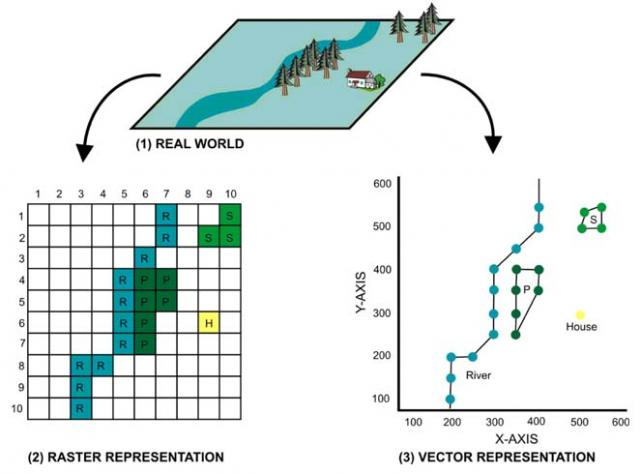
\includegraphics[width=0.8\textwidth]{pics/RasterVectorPreview}
\caption{Difference between raster and vector data representation}
\label{pic:RasterVector}
\end{figure}

Both representations carry various set of advantages and disadvantages. These will be described in the following subsections.

% http://data.geocomm.com/helpdesk/formats.html
\subsection{Raster representation}
Raster type formats consist of equally sized cells arranged in rows and columns to construct the representation of space. Individual cell contains an attribute value and location coordinates. Together they create images of point, line, area, network or surface.

\paragraph*{Advantages}
\begin{itemize}[noitemsep]
\item Easy and "cheap" to render
\item Represent well both discrete (urban areas, soil types) and continuous data (elevation)
\item Grid nature provides suitability for mathematical modeling or quantitative analysis
\end{itemize}

\paragraph*{Disadvantages}
\begin{itemize}[noitemsep]
\item Large amount of data
\item Scaling required between layers
\item Possible information loss due to generalization (static cell size)
\item Difficult to establish network linkage
\end{itemize}

\subsection{Vector representation}
Vector type formats uses vertices as a basic unit. Vertex consist of x and y coordinates to determine it's position. Using vertices it is possible to create any shape to describe any object. One vertex create point, two can create line etc. Object created by vertices may contain additional attributes describing the feature.

\paragraph*{Advantages}
\begin{itemize}[noitemsep]
\item Topology nature
\item Compact data structure
\item Easy to maintain
\item Bigger analysis capability
\end{itemize}

\paragraph*{Disadvantages}
\begin{itemize}[noitemsep]
\item For effective analysis static topology needs to be created
\item Every update rebuilding topology is necessary
\item Continuous data not effectively represented
\end{itemize}

\section{Summary -- data usage}
Most of the official European sources (EuroGeographics, EPSON) require filling a form for each download of data. This process can be bottom neck for maintenance part of the application while updating the data would take big amount of time and required additional functionality. 

%Next very significant part of the choice is the data format. As was said in subsection HERE_ADD_SECTION well 

\chapter{Analysis and design}

\section{Data storage}
%TODO
Since the data source and format question is resolved, next step is to decide the representation of graph in the memory. During the history of graph theory there are three main representations to choose from. In following subsections we will take closer look at all three options.

\subsection{Adjacency list}
Adjacency list stores graph as a list of vertices. Each vertex then contains an information about it's adjacent vertices in form of linked list. Adjacency list is easy to implement and use. All vertices in a graph are mapped onto the array of pointers referencing to a first node of a linked list. In case a vertex does not have the adjacent vertices its pointer is set to null. An example of adjacency list for a simple graph can be found in Figure \ref{pic:AdjacencyList}. 

\begin{figure}[h]
\centering
\includegraphics[width=0.8\textwidth]{pics/GraphRep}
\caption{Representation of graph using adjacency list}
\label{pic:AdjacencyList}
\end{figure}


\subsection{Adjacency matrix}
\label{subsec:AdjMatrix}
Adjacency matrix is defined as matrix of a size $|V(G)| \times |V(G)|$, where $V(G)$ is a set of all vertices in graph $ G $. Values within the matrix depends on the type of the graph. Generally for unweighted graph we define adjacency matrix as a $\textbf{A}(G)=[a_{ij}] $, where $a_{ij}$ is the number of edges joining $v_i$ and $v_j$. If the graph is weighted, the values are from interval $\langle 0, \infty ) $, where $0$ means two vertices are not adjacent and any non-zero value means they are adjacent with an edge cost of that value\cite{Bondy76}. Although between every two vertices must exist 1 edge at most.
For the graph G in the Figure \ref{pic:AdjacencyList} adjacency matrix $\textbf{A}$ looks exactly like:
\[
\textbf{A}(G) =
\kbordermatrix{
 & v_{0} & v_{1} & v_{2} & v_{3} & v_{4} \\
v_{0} & 0 & 1 & 0 & 0 & 1 \\
v_{1} & 0 & 0 & 1 & 1 & 0 \\
v_{2} & 0 & 0 & 0 & 1 & 0 \\
v_{3} & 0 & 0 & 0 & 0 & 0 \\
v_{4} & 0 & 0 & 0 & 1 & 0 	
}
\]
Rows and columns represent vertices of a graph. In my case first row and first column represents vertex $0$, second row and column vertex $1$ etc. Value in third row and fourth column means that vertex 2 is adjacent with vertex 3. % As an interesting observation 
It is noticeable that because my example graph is directed, adjacency matrix is not symmetric. %TODO possible extent of directed/undirected graphs

\subsection{Incidence matrix}
Incidence matrix is very similar to adjacency matrix, but instead of showing relations between vertices themselves it represents relation between vertices and edges. Which means size of incidence matrix is $|V(G)| \times |E(G)|$, where $V(G)$ is a set of all vertices and $E(G)$ is set of all edges in graph $ G $. Incidence matrix of graph G is then $\textbf{M}(G) = [m_{ij}]$, where $m_{ij}$ is the number of times (0, 1 or 2 in case of loop) that vertex $v_i$ and edge $e_j$ are incident\cite{Bondy76}.

Interesting case is incidence matrix for directed graph. In that case the sign of the value within matrix $\textbf{M}$ describes the orientation of the edge. Given the edge $e = (x, y)$ then in the row of vertex $x$ and corresponding column for edge $e$ is value is positive and in the row of vertex $y$ and corresponding column for edge $e$ is negative.
For the graph G in the Figure \ref{pic:AdjacencyList} incidence matrix $\textbf{M}$ looks exactly like:

\[
\textbf{M}(G) =
\kbordermatrix{
 & e_{0} & e_{1} & e_{2} & e_{3} & e_{4} & e_5 \\
v_{0} & 1  & 0  & 1  & 0  & 0  & 0 \\
v_{1} & -1 & 1  & 0  & 1  & 0  & 0 \\
v_{2} & 0  & -1 & 0  & 0  & 1  & 0 \\
v_{3} & 0  & 0  & 0  & -1  & -1  & -1 \\
v_{4} & 0  & 0  & -1 & 0  & 0  & 1
}
\]

\subsection{List and matrix comparison}
Both matrices and list stores equivalent information about the graph. From incidence matrix we can read which two edges share the same vertex (they are incident) and from adjacency matrix which two vertex are connected with an edge. Adjacency list stores for each vertex node edge information in form of linked list which brings two main benefits. 

First benefit is adding a new vertex takes constant time. 

My application needs to be able to store graph with a lot of vertices and edges using minimum size.

\subsection{Sparse matrix}
In mathematics matrices can be divided into two groups: sparse matrices and dense matrices. The definition might sound somehow vague, but sparse matrix is matrix containing huge amount of zero elements. Dense matrix is the exact opposite: containing very few zero elements. In previous subsections it is noticeable that each of the matrices (adjacency and incidence) consist of a lot of zero elements and only few are actually useful values.

The amount of non-zero elements in the adjacency or incidence matrix depends purely on degree of vertices in the graph. In both types of matrices, each row serve as a vertex and within non-zero values represent edges incident to the vertex. Depending on if the graph is directed or undirected the amount of non-zero elements in adjacency matrix will differ. Incidence matrix does not change its number, because it differs only in sign of the value. 

For undirected graphs the number of non-zero elements equals to $$ \sum_{v \in V} \textrm{deg(v)} = 2|E| $$ where $E$ set of all edges and $V$ set of all vertices in graph. Same applies to the directed graph for incidence matrix. For directed graph and adjacency matrix we can observe that the number of non-zero elements depends on amount of the outgoing edges $\Rightarrow$ out-degree, which is 
$$ \sum_{v \in V} \textrm{deg\textsuperscript{--}(v)} = |E| $$ where $E$ is set of all edges, $V$ is set of all vertices in graph and $deg\textsuperscript{--}(v)$ function returns number of outgoing edges from the vertex $v$.

The reason why I mentioned sparse matrix in the first place is that there are functions and operations which could be done above the sparse matrices. The main motivation for this section are the storage schemes in which sparse matrix could be stored. Using storage scheme enables all the advantages of the regular matrix representation with significantly less memory usage since only the non-zero elements are being stored.

According to %TODO cite Yasaad
there are X storage schemes. 

Coordinate format belongs to the simplest storage schemes of sparse matrices. The data structure consists of three arrays: an array containing all the (real or complex) values of the non-zero elements of the original matrix in any order, an integer array containing their row indices and a second integer array containing their column indices. All three arrays are of length $N$, which is the number of non-zero elements.

Let us take a look at adjacency $\textbf{A}$ matrix from section \ref{subsec:AdjMatrix}. Clearly this matrix contains less non-zero elements, therefore it is an example of sparse matrix. Using coordinate format matrix $\textbf{A}$ looks the following way:

$$
\begin{array}{c}
AA:
\begin{array}{|c|c|c|c|c|c|}
 \hline
 1 & 1 & 1 & 1 & 1 & 1 \\
 \hline
\end{array}
\\ \\
IR:
\begin{array}{|c|c|c|c|c|c|}
 \hline
 0 & 1 & 2 & 0 & 1 & 4 \\
 \hline
\end{array}
\\ \\
IC:
\begin{array}{|c|c|c|c|c|c|}
 \hline
 4 & 2 & 3 & 1 & 3 & 3 \\
 \hline
\end{array}
\end{array}
$$

Array $AA$ stores values of non-zero elements, array $IR$ stores the row index of the corresponding element and array $IC$ stores the column index of the corresponding element. The memory needed for storing matrix is now only $3N$ instead of the original $N^2$.

If the elements inside array $AA$ are listed by row, the array $IR$ could be transformed to store only indices of the beginning of each row instead. The size of newly defined array $IR$ is then $n+1$, where $n$ is number of rows in original matrix. On the last position ($+1$) is being written the number on non-zero elements within the original matrix. It also may be represented as address, where fictional $n+1$ row begins. 

Array $\textbf{A}$ then would be by this scheme described in the following way:

$$
\begin{array}{c}
AA:
\begin{array}{|c|c|c|c|c|c|}
 \hline
 1 & 1 & 1 & 1 & 1 & 1 \\
 \hline
\end{array}
\\ \\
IR:
\begin{array}{|c|c|c|c|c|c|}
 \hline
 0 & 2 & 4 & 5 & 5 & 6 \\
 \hline
\end{array}
\\ \\
IC:
\begin{array}{|c|c|c|c|c|c|}
 \hline
 1 & 4 & 2 & 3 & 3 & 3 \\
 \hline
\end{array}
\end{array}
$$



The transformation of the $IR$ array and listing elements inside $AA$ by row is called Compressed Sparse Row (CSR) format. In scientific computing CSR format is most commonly used for vector-matrix multiplication while having low memory usage. On the other hand coordinate format excels with it\'s simplicity and flexibility.
Compressed Sparse Row format through the years develops in many number of variations. 
While storing columns instead of rows, we create a new scheme known as Compressed Sparse Column (CSC) format.

The last scheme I would like to point out is the Ellpack-Itpack format which is very popular on vector machines. The Ellpack-Itpack format stores matrix in two 2-dimensional arrays of the same size $n \times N_{mpr}$, where $n$ is the number of rows of the original matrix and $N_{mpr}$ represents maximum of non-zero elements per row. The first array contains non-zero elements of original matrix. If the number of non-zero elements is less then the $N_{mpr}$, the rest of the row is filled with zeroes. The second array stores the information about the column in which specific non-zero element is located. For each zero in the first array can be added any number.
The Ellpack-Itpack format for the matrix TODO is TODO.

\section{Definitions and problem description}

\subsection{Directed graph}
A directed \textit{graph} $G$ is a pair $(V, E)$, where $V$ is a finite set of \textit{vertices} and $E \subseteq V \times V$ are the $edges$ of a graph $G$. Throughout this paper, the number of vertices $|V|$ is denoted by $N$ and the number of edges $|E|$ is denoted by $m$. A $path$ in $G$ is a sequence of vertices $v_1, v_2 \dots ,v_k$ such that $(v_i,v_{i+1}) \in E$ for all $1 \leq i < k$. A path with $v_1 = v_k$ is called a $cycle$. A graph (without multiple edges) can have up to $n^2$ edges. We call a graph \textit{sparse}, if $m \in O(n)$. We assume that we are given a layout $L : V \to R^2$ of the graph in the Euclidean plane. For ease of notation, we will identify a node $v \in V$ with its location $L(v) \in R2$ in the plane.

\subsection{Shortest path problem}
Let $G = (V, E)$ be a directed graph whose edges are weighted by a function $f(e): E \to R$. We interpret the weights as edge lengths in the sense that the length of a path is the sum of the weights of its edges. The (single-source single-target) shortest-path problem consists in finding a path of minimum length from a given source $s \in V$ to a given target $t \in V$. Note that the problem is only well defined for all pairs, if $G$ does not contain negative cycles. If there are negative weights, but not negative cycles, it is possible, using Johnson’s algorithm [Johnson 1977], to convert in $O(n_m + n^2 \log n)$ time the original edge weights $f(e): A \to R$ to non-negative arc weights  : A → R+ 0 that result in the same shortest paths. Hence, in the rest of the paper, we can safely assume that edge weights are non-negative. Throughout the paper we also assume that for all pairs $(s,t) \in V \times V $ the shortest path from $s$ to $t$ is unique. Kranakis et al. [1995], for instance, gave a detailed description on how one can transform any graph into such a unique shortest-path graph.


\subsection{Dijkstra algorithm}

\section{User interface design}

\chapter{Realisation}

\setsecnumdepth{part}
\chapter{Conclusion}


\bibliographystyle{iso690}
\bibliography{mybibliographyfile}

\setsecnumdepth{all}
\appendix

\chapter{Acronyms}
% \printglossaries
\begin{description}
	\item[CERCO] Comit{\' e}e Europ{\' e}en des Responsables de la Cartographie Officielle\item[GUI] Graphical user interface
	\item[DEM] Digital Elevation Model
	\item[ERDF] European Regional Development Fund
	\item[ESPON] European Observation Network for Territorial Development and Cohesion
	\item[GIS] Geographic information systems	
	\item[MEGRIN] Multi-purpose European Ground Related Information Network
	\item[OSM] OpenStreetMaps
	\item[XML] Extensible markup language
	
	
\end{description}


\chapter{Contents of enclosed CD}

%change appropriately

\begin{figure}
	\dirtree{%
		.1 readme.txt\DTcomment{the file with CD contents description}.
		.1 exe\DTcomment{the directory with executables}.
		.1 src\DTcomment{the directory of source codes}.
		.2 wbdcm\DTcomment{implementation sources}.
		.2 thesis\DTcomment{the directory of \LaTeX{} source codes of the thesis}.
		.1 text\DTcomment{the thesis text directory}.
		.2 thesis.pdf\DTcomment{the thesis text in PDF format}.
		.2 thesis.ps\DTcomment{the thesis text in PS format}.
	}
\end{figure}

\end{document}
